\documentclass{report}
\usepackage[utf8]{inputenc}
\usepackage{graphicx}
\usepackage{ngerman}
\usepackage{url}
\usepackage{amsmath}
\usepackage{wrapfig}
\usepackage{subscript}
\usepackage{eurosym}
\usepackage{biblatex}
\usepackage{url}
\usepackage{color}
\usepackage{listings}
\usepackage{hyperref}

\definecolor{mygreen}{rgb}{0,0.6,0}
\definecolor{mygray}{rgb}{0.5,0.5,0.5}
\definecolor{mymauve}{rgb}{0.58,0,0.82}

\let\origitemize\itemize
\def\itemize{\origitemize\itemsep0pt}

\lstset{ 
  backgroundcolor=\color{white},   
  basicstyle=\ttfamily\footnotesize,          
  breakatwhitespace=false,         
  breaklines=true,  
  commentstyle=\color{mygreen}, 
  escapeinside={\%*}{*)}, 
  extendedchars=true,             
  keepspaces=true,                 
  keywordstyle=\color{blue},
  language=Octave,                 
  morekeywords={html, head, body, link},
  numbers=left,                   
  numbersep=15pt,                  
  numberstyle=\tiny\color{mygray}, 
  showspaces=false,                
  showstringspaces=false,          
  showtabs=false,                  
  stringstyle=\color{mymauve},
  tabsize=2,
  title=\lstname,
  captionpos=b
}

\lstdefinelanguage{JavaScript}{    %Java Script Language Definition 
  keywords={typeof, new, true, false, catch, function, return, null, catch, switch, var, if, in, while, do, else, case, break},
  ndkeywords={class, export, boolean, throw, implements, import, this},
  sensitive=false,
  comment=[l]{//},
  morecomment=[s]{/*}{*/},
  morestring=[b]',
  morestring=[b]"
}

\renewcommand*\lstlistingname{Codebeispiel}    %Rename Listings

\bibliography{doku}


\renewcommand*\thesection{\arabic{section}}
\begin{document}

\title{Waking Wind}
\author{Thorsten Schaeff \and Daniel Grie\ss haber}
\maketitle
\tableofcontents

\renewcommand\bibname{Referenzen}

\printbibliography


\begin{abstract}
\glqq Waking Wind\grqq ~ist ein Webservice der Windsportler mit Echtzeit Wetterdaten versorgt.
Der Slogan „real-time wind data from anywhere to everywhere“ beschreibt unseren Fokus auf die möglichst einfache Erfassung von Daten selbst von abgelegenen Orten sowie das möglichst einfache Abrufen der Daten auch von unterwegs.

In dieser Dokumentation soll der Prozess von der Idee zum fertigen Produkt aufgezeigt werden.
\end{abstract}

\section{Die Wetterstation}
Bei der verwendeten Wetterstation handelt es sich um eine CTW-600 der Firma Chillitec GmbH\cite{CTW-600}. Diese wurde wegen ihres geringen Preises und der Vielzahl an Messgeräten die sie zur Verfügung stellt ausgewählt. Sie besteht aus 2 Komponenten, dem Außensensor und der Basisstation. Der Außensensor bietet folgende Sensoren:
\begin{wrapfigure}{r}{0.46\textwidth}
    \begin{center}
        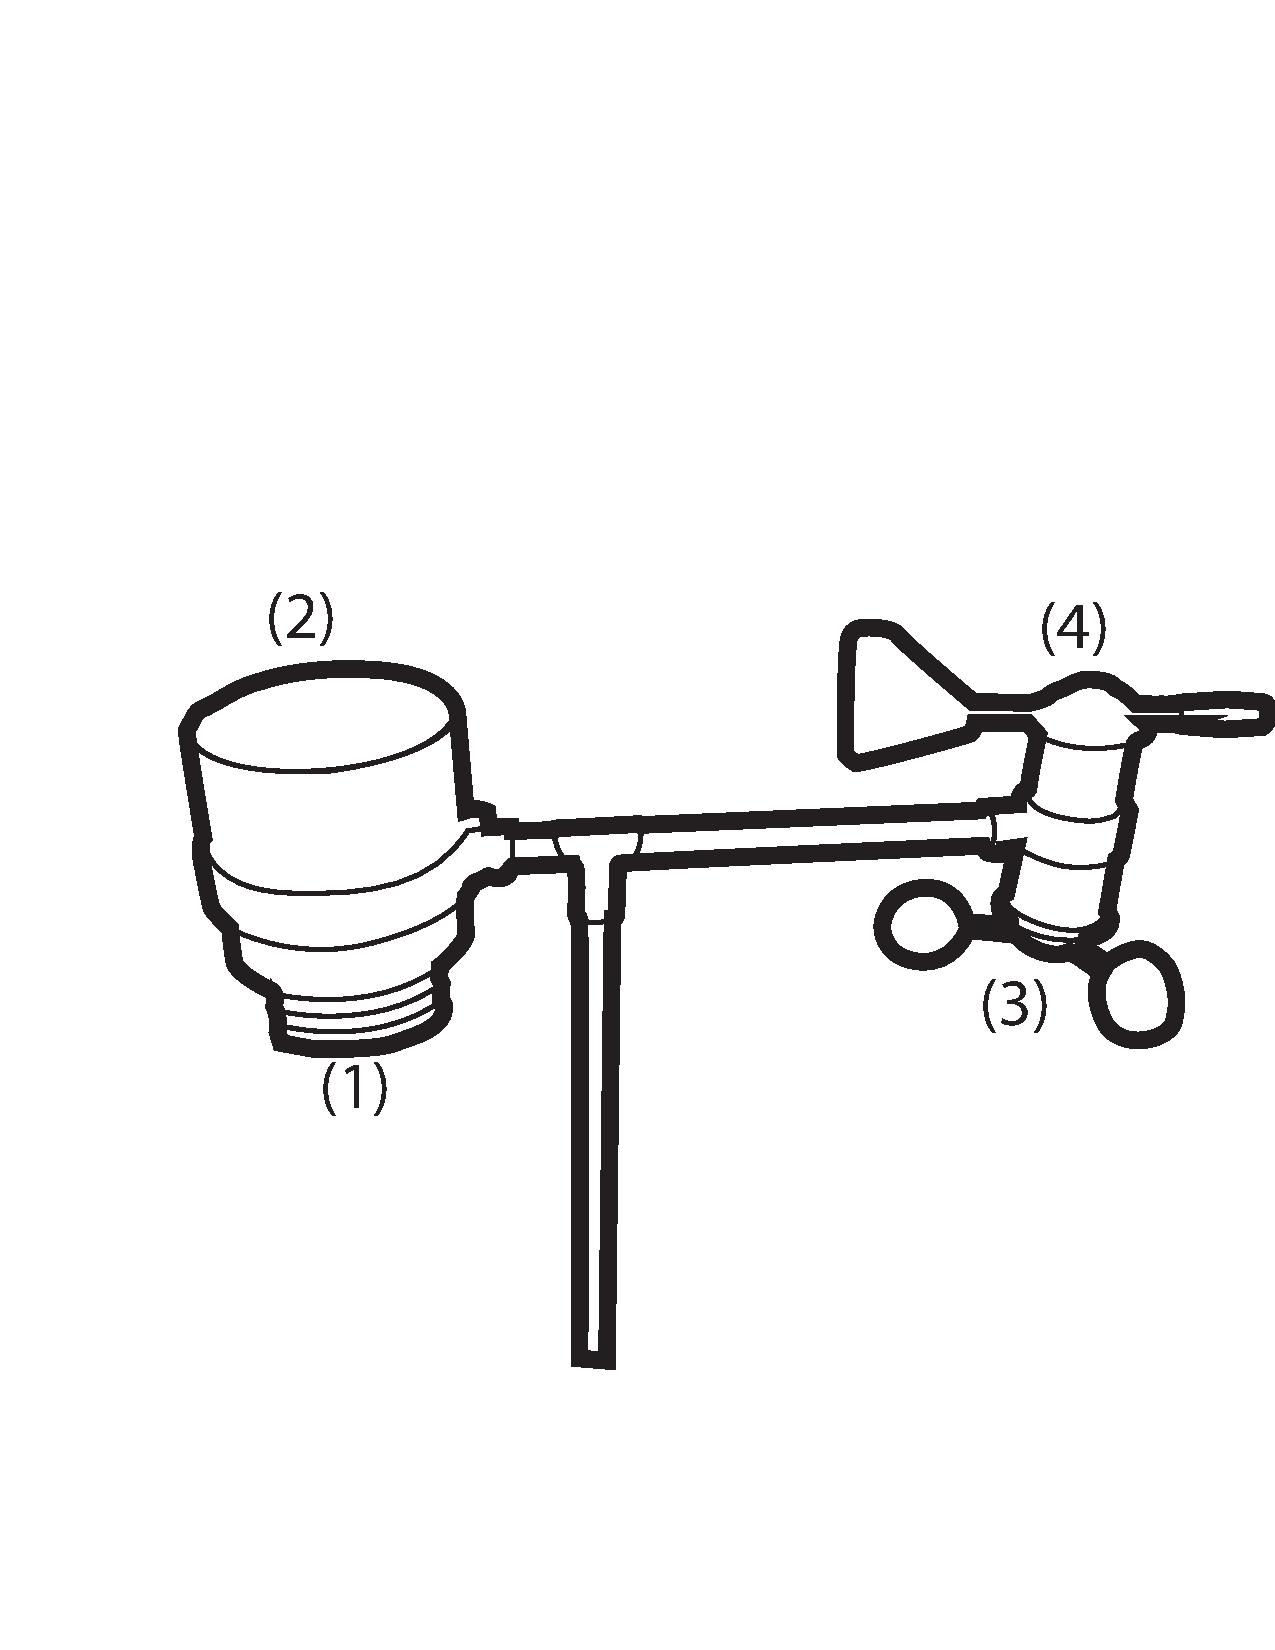
\includegraphics[width=0.45\textwidth]{Bilder/Wetterstation.pdf}
    \end{center}
    \vspace{-50pt}
\end{wrapfigure}

\begin{itemize}
    \item (1) Temperatursensor
    \item (1) Luftfeuchtigkeitssensor
    \item (2) Regenfallsensor
    \item (3) Anemometer
    \item (4) Windrichtungssensor
\end{itemize}

Ein weiterer Vorteil dieser Wetterstation war die Kabellose Übertragung der Daten über das 433MHz Band. Dies ermöglichte das einfache Abgreifen der Daten.


\section{Das Protokoll der Wetterstation}
\begin{wrapfigure}{r}{0.5\textwidth}\centering
    \begin{center}
        \includegraphics[width=0.48\textwidth]{Bilder/Receiver.png}
    \end{center}
\end{wrapfigure}
Der erste Schritt bestand in der Demodulation des 433MHz, amplitudenmodulierten Signals. Dieser Schritt gestaltete sich deutlich einfacher als zunächst angenommen, da die Basisstation ein, auf die Frequenz abgestimmtes, Empfangsmodul auf seine Hauptplatine aufgelötet hatte. Da die Basisstation nicht weiter benötigt wurde, konnte dieses Modul abgelötet und als Demodulator für das Signal verwendet werden. Das Modul bietet 3 Pins in Form einer Stiftleiste. Diese Pins haben folgende Funktion:

\begin{itemize}
    \item (1) Vcc (Positive Stromversorgung)
    \item (2) GND (Masse)
    \item (3) SIG (Daten Pin)
\end{itemize}
Zusätzlich wurde noch hinzugefügt:
\begin{itemize}
    \item (4) ANT (Verbindung zur Antenne)
\end{itemize}
Mithilfe eines Voltmeters war die Pinbelegung leicht herauszufinden. 

\subsection{Abgreifen der Daten}
Zum Abgreifen der Daten wurden zunächst mehrere Möglichkeiten evaluiert. 
Die erste Variante bestand darin ein Arduino Leonardo\cite{ArduinoLeonardo} mit einer speziellen Implementierung des offenen SUMP Logic Analyzer Protocols\cite{SUMP} zu verwenden. Nach einigen Testversuchen zeigte sich, dass die Buffergröße des Leonardos zu klein war und die serielle Übertragungsrate des virtuellen USB Ports zu gering war um die Datenrahmen der Wetterstation aufzunehmen. 

Eine naheliegende Alternative wären professionelle Logik Analysatoren, welche allerdings preislich ein vielfaches eines Arduino Leonardo kosten.

Durch die fehlerhaften Mitschnitte der Daten hat sich jedoch gezeigt, dass die einzelnen Signale in einer Abfolge von mindestens $400\mu s$ aufeinander folgen. Daraus ergab sich eine nötige Abtastrate bei der Analyse nach dem Abtastheorem von Nyquist\cite{Nyquist1928} und Shannon von:
\begin{equation*}
    \frac{1}{400\mu s}*2=5kHz
\end{equation*}
Durch dieses Wissen war es möglich die Daten mithilfe einer Soundkarte, welche im Normalfall über eine Samplingrate von $44.1kHz$ verfügt, aufzuzeichnen. 

Da das Empfangsmodul mit einer Spannung von $5V$ arbeitet, der Line Anschluss einer Soundkarte allerdings einen Bezugspegel von $0.5V$ benötigt, wurde ein Transistor zur Entkopplung eingefügt.
\begin{figure}[!htbp]
    \begin{center}
        \includegraphics[width=7cm]{Bilder/433MHZAnschluss.pdf}
    \end{center}
    \label{433MHZAnschluss}
    \caption{Entkopplung des Signals mithilfe eines Transistors}
\end{figure}

Die Datenrahmen wurden mit der freien Audio Software Audacity\cite{Audacity} aufgezeichnet und ausgewertet.


\subsection{Signal}
Bei Auswertung des Signals fiel auf, dass das Signal zusätzlich mit einer Pulsweitenmodulation codiert war. Dabei repräsentiert ein hohes, kurzes Signal eine logische $1$ und ein hohes, langes Signal eine logische $0$. Die Pause zwischen den Signalen ist immer gleich lang und dient lediglich zur Abgrenzung der logischen Pegel. Durch Vergleich mehrerer aufgezeichneter Datenrahmen konnte folgendes Wissen über die Pulslängen hergeleitet werden:

\begin{figure}[!h]
    \begin{center}
        \includegraphics[width=10cm]{Bilder/PWMSchematic.pdf}
    \end{center}
    \caption{Illustration eines PWM Signals}
    \label{PWMSchematic}
\end{figure}

\begin{table}[!h]
\begin{center}
    \begin{tabular}{l c@{ - }c}\hline
        \text {Ausdruck}& \multicolumn{2}{c}{Dauer $t\textsubscript{i} [\mu s]$}\\\hline
        \hline
        1                 &    400 & 621\\
        N (Pause)         &    805 & 1150\\
        0                 &    1495 & 1840
    \end{tabular}
    \caption{Pulslängen der logischen Werte}
    \label{tab:timing}
    \end{center}
\end{table}


Dieses Wissen Abbildung war auch für das spätere Design des Empfängers notwenig, da pulsweitenmodulierte Signale normalerweise mit einem Tiefpassfilter gefiltert werden. Durch die diskrete Anzahl an möglichen Pulslängen ist dies allerdings nicht nötig, sondern das Signal kann auch in Echtzeit durch ein diskretes Programm demoduliert werden.


\subsection{Protokoll}
Die Datenrahmen besitzen eine Länge von 88 Bit. Diese Rahmen mussten den folgenden Informationen zugeordnet werden:

\begin{itemize}
    \item Temperatur
    \item Luftfeuchtigkeit
    \item Regenfall
    \item Windgeschwindigkeit
    \item Windrichtung
\end{itemize}
Außerdem hat sich im Verlauf des Reverse Engineerings gezeigt dass zusätzlich noch folgende Informationen von der Wetterstation übertragen werden:
\begin{itemize}
    \item Eindeutige ID des Au\ss ensensors
    \item Batterieladungszustand des Au\ss ensensors
    \item Prüfsumme aller Daten
\end{itemize}
Die Zuordnung der Daten erfolgte iterativ in folgenden Schritten
\begin{enumerate}
    \item Aufzeichnung und Demodulation eines Datenrahmens
    \item Aufzeichnung der Daten an der Wetterstation
    \item Einen gezielten Stimuli auf einen der Sensoren der Wettertstion geben
    \item Aufzeichnen eines weiteren Datenrahmens und der Daten der Basisstation
    \item Finden der unterschiedlichen Stellen zwischen den beiden Datenrahmen
    \item Assoziationsanalyse mit der gefundenen Differenz der Datenpakete und den Daten der Basisstation
\end{enumerate}
Letztlich ergab sich folgende Tabelle, mit deren Hilfe das Protokoll beschrieben werden kann. Dabei werden die Bits in ihrer chronologischen Reihenfolge in der sie von dem Au\ss ensensor gesendet werden durchnummeriert.

\renewcommand{\arraystretch}{1.4}
\begin{center}
    \begin{tabular}{clp{3.5cm}l}\hline
        \text {Bits} & \text{Bedeutung} & \text{Umrechnung} & \text{Default Wert} \\\hline
        \hline
        0 - 9 & Synchronisation & - & $1111111110\textsubscript{2}$\\
        11 - 13 & Batterieladungszustand & $Wert\textsubscript{10} = [0 - 15]$ & -\\
        14 - 19 & Eindeutige ID des Aus\ss ensensors & - & -\\
        20 - 21 & Keine Bedeutung & - & $00\textsubscript{2}$\\
        22 - 31 & Temperatur & $T[\,^{\circ}\mathrm{C}] = \frac{Wert\textsubscript{10} - 400}{10}$ & -\\
        32 - 39 & Luftfeuchtugkeit & $\varphi[\%] = Wert\textsubscript{10}$\\
        40 - 55 & Windgeschwindigkeit & $v[\frac{km}{h}] = \frac{Wert\textsubscript{10}}{240}$ & -\\
        56 - 71 & Regenfall & $V[\frac{mm}{m\textsuperscript{2}}] = Wert\textsubscript{10} \cdot 0.3$ & -\\
        72 - 75 & Keine Bedeutung & - & $00\textsubscript{2}$\\
        76 - 79 & Windrichtung & $Wert\textsubscript{10}$Anordnung wie Windrose, 0=Norden & -\\
        80 - 88 & Prüfsumme & \emph{unbekannt} & - \\
    \end{tabular}
\end{center}
\renewcommand{\arraystretch}{1}

\begin{wrapfigure}{r}{3cm}
    \begin{center}
        \includegraphics[width=2.9cm]{Bilder/Windrose.pdf}
        \vspace{-1cm}
    \end{center}
\end{wrapfigure}
Die Windrichtung ist im Uhrezeigersinn durchnummeriert und in 8 Teile unterteilt. Für die 16tel Teile wurden Platzhalter freigelassen, jedoch werden diese nicht von der Wetterstation genutzt.


Um herauszufinden wie sich die Prüfsumme berechnet wurden folgende Algorithmen auf mehreren Datenrahmen getestet:
\begin{itemize}
    \item CRC-8
    \item Summe über alle Bytes (Überlaufe ignorieren)
    \item Verschiedene Kombinationen von XOR Gattern auf Byte Basis
\end{itemize}
Obwohl es nicht gelang den tatsächlich verwendeten Algorithmus zu identifizieren, ist die Lösung der XOR Gatter - aufgrund des sehr geringen Berechnungsaufwandes und der einfachen Realisierung in Hardware - die Naheliegendste.

\section{Empfänger}
Die Aufgabe des Empfängers ist es, das Signal der Wetterstation zu empfangen, zu demodulieren, zu interpretieren und in der Datenbank persistent zu speichern. Sekundäre Ziele waren eine möglichst günstige Fertigung, sowie die Unabhängigkeit von der Umgebung und ggf. der Infrastruktur.

Für die Umsetzung der Ziele wurde der Empfänger in 2 Module aufgeteilt; das Empfangsmodul, dessen Aufgabe der Empfang und die Demodulation des Signals ist, und einer weiteren aktiven Komponente für die Interpretation und Übertragung der Daten. 

Für den Prototyp nahm ein Raspberry PI\cite{RasPi} die Rolle der zweiten Komponente ein, da dieser durch seinen geringen Stromverbrauch von ca. $2W$ und den geringen Anschaffungspreis von ca. \euro{35} die Kosten für die Inbetriebnahme und den Betrieb einer Station nicht unnötig in die Höhe treibt. 

Das Empfangsmodul musste aufgrund der speziellen Anforderungen selbst entwickelt werden. Dabei stand auch die Minimierung der Kosten im Vordergrund.

\subsection{Empfangsmodul}
Das Herz des Empfangsmoduls bildet ein ATTiny 45 Mikrocontroller\cite{ATtiny45} der mit einem internen $8MHz$ Quarzoszillator arbeitet. Auf einen externen Quarz wurde, aus Kostengründen und weil der ATTiny nur 5 Input/Output Pins hat, verzichtet. Ein externer Quarz hätte 2 dieser Pins für die Taktversorgung bereits belegt. Für die Einspeisung des Signals wurde der $433MHz$ Empfänger der Basisstation verwendet und an \verb+PB2+ des Mikrocontrollers angeschlossen. 

Aufgrund des fehlenden Hardware UART für die serielle Übertragung musste ein minimaler Software UART (siehe Seite \pageref{SoftwareUart}) implementiert werden. Die Daten werden über diesen an einen USB auf UART Adapter gesendet, der auf seiner USB Seite einen virtuellen, seriellen Port zur Verfügung stellt, auf dem die Daten nach dem Empfang ausgelesen werden können.

Für die Funktionsanzeige wurde an den noch übrigen \verb+PB1+ und \verb+PB3+ eine zweifarbige LED angebracht. Diese leuchtet beim Empfang eines $433MHz$ Signals gelb und blinkt bei erfolgreichem Empfang eines Datenrahmens rot.

\subsubsection{Verbesserung der Empfangsqualität}
Für die Verbesserung der Empfangsqualität wurde die alte Drahtantenne des Basisstationsempfängers durch einen SMA-Anschluss ersetzt. Da diese der Standart für WLAN Antennen sind, haben sie den Vorteil, dass sie sehr preiswert in der Anschaffung sind. Zusätzlich wurde eine alte WLAN Antenne für den Empfang von $433MHz$ Signalen umgerüstet. Es gibt zwar auch spezielle $433MHz$ Antennen, jedoch sind diese wegen ihrer geringen Verbreitung sehr teuer.

Für die Umrüstung wurde die Antenne geöffnet und auf die passende Länge gekürzt. Die Wellenlänge eines $433MHz$ Signals berechnet sich wie folgt:
\begin{equation*}
    \lambda = \frac{c}{f} = \frac{3 \cdot 10\textsuperscript{8}\frac{m}{s}}{433MHz} \approx 69.23cm
\end{equation*}
Aufgrund des Platzmangels im Gehäuse der WLAN Antenne wurde die Antenne noch auf $\frac{\lambda}{8} \approx 8.65cm$ gekürzt.


\begin{figure}[!h]
    \begin{center}
        \includegraphics[width=13cm]{Bilder/board_schematic.pdf}
    \end{center}
    \caption{Schematik des Empfängers}
    \label{schematik}
\end{figure}

\subsubsection{Das Empfangen der Daten}
Das Hauptprogramm, das auf dem Mikrocontroller läuft arbeitet nach dem Schema in [Abbildung \ref{ablauf}].
\begin{figure}[!htb]
    \begin{center}
        \includegraphics[width=8cm]{Bilder/EmpfangsmodulActivity.pdf}
    \end{center}
    \caption{Ablaufdiagramm des Hauptprogramms}
    \label{ablauf}
\end{figure}

Dabei ist anzumerken, dass es durch das kritische Timing beim Empfang des Signals nicht möglich war, die ankommenden Bits direkt zu übersetzen. Deshalb werden zuerst die Timerwerte zwischengespeichert und nach erfolgreichem Empfang eines Rahmens diese Werte mit Hilfe der [Tabelle \ref{tab:timing}] übersetzt. 

Wird beim Empfang festgestellt, dass zwischen zwei Pegelwechseln die Zeit größer der maximalen Länge für eine logische $0$ überschritten wird, wird der Empfang abgebrochen, da es sich nicht um das Signal der Wetterstation handelt.

\subsubsection{Der Software UART}\label{SoftwareUart}
Für die Übertragung der Daten vom Mikrocontroller zum USB auf UART Adapter war eine eigene Implementierung nötig, da der Mikrocontroller keine Hardware Implementierung des \textbf{U}niversal \textbf{A}synchronus \textbf{R}eciever and \textbf{T}ransmitter bereitstellt.  

Mikrocontroller, die diese Schnittstelle bereitstellen, sind mit deutlich mehr Funktionen und Input/Output Ports ausgestattet. Das erhöht sowohl den Preis, als auch die Baugrö\ss e dieser Chips.

Die eigene Implementierung beschränkt sich auf das Senden der Daten, da nur die Simplex Kommunikation in Richtung der Schnittstelle vorgesehen ist. Dabei wird die Datenleitung, solange keine Übertragung stattfindet, durch den internen PullUp Widerstand des ATTiny auf einem Pegel von $+5V$ gehalten. Die Übertragung erfolgt Byteweise. Dabei wird am Anfang jedes Bytes die Leitung auf logisch $0$ ($0V$) gezogen. Danach erfolgt die Übertragung der Bits durch entprechendes senken auf $0V$ oder halten auf $+5V$. Am Ende des Bytes wird die Leitung für das Stoppbit wieder auf $+5V$ gehalten.

\begin{figure}[!htb]
    \begin{center}
        \includegraphics[width=\textwidth]{Bilder/UART.pdf}
    \end{center}
    \caption{Beispielverlauf der Übertragung über UART}
    \label{UART}
\end{figure}

Da bei dieser Art der Übertragung das Timing wichtig ist, muss im Vorfeld geklärt werden, wielange die Dauer $t\textsubscript{i}$ eines Bits (Symbol) ist. Durch Versuche zeigte sich, dass die höchste Symbolrate (Baudrate) bei $38400 Baud$ liegt, ohne dass es zu Übertragungsfehlern durch Überlastung des Mikrocontrollers kommt. Dadurch ließ sich die Anzahl der Takte zwischen den Flankenwechseln ($t\textsubscript{i}$) mit folgender Formel berechnen:

\begin{equation*}
    \frac{IO Clock}{Prescaler \cdot 1MHz} \cdot \frac{1MHz}{BAUD} = \frac{8MHz}{1 \cdot 1MHz} \cdot \frac{1MHz}{38400 Baud} \approx 208
\end{equation*}

\subsection{Herstellung des Prototypen}
Während der Evaluations- und Implementierungsphase wurde die Schaltung lediglich auf einem Breadboard (Steckbrett) betrieben. Für den produktiven Einsatz musste aber eine dauerhafte und stabilere Lösung gefunden werden.

Aus diesem Grund wurde zusätzlich zur Schematik des Empfängers ein \textbf{P}rinted \textbf{C}ircuid \textbf{B}oard Layout erstellt. Dabei wurde für günstige Konstruktionspreise darauf geachtet, dass das Layout der Leiterplatte nur auf einer Seite bearbeitet werden muss.

\begin{figure}[!htb]
    \begin{center}
        \includegraphics[width=11cm]{Bilder/board.pdf}
    \end{center}
    \caption{Das PCB Layout}
    \label{board}
\end{figure}

Bei weiteren Versionen des Layouts könnte noch die Komponente \verb+JP2+ in der Mitte entfernt werden, da diese nur zur Programmierung des Chips gebraucht wird. Ausserdem könnte der Anschluss für die Antenne oben links (\verb+ANT+ und \verb+GND+) weiter in die Mitte verschoben werden, so dass dieser besser gegen elekromagnetische Störerscheinungen durch die Masseplatte abgeschirmt wird.

Als nächstes wurde das zweidimensionale Layout in einer 3D Software modelliert um eine bessere Vorstellung der Ma\ss e zu bekommen und um ein passendes Gehäuse auswählen zu können (Abbildung \ref{board3d}).

Zur Herstellung der Prototyp Platine wurde das Tonertransferverfahren auf ein zugeschnittenes Stück einseitig mit Kupfer beschichtete Epoxydplatte angewendet. Dabei geht man in folgenden Schritten vor:
\begin{enumerate}
    \item Reinigen der Kupferfläche von Fetten mithilfe von Ethanol
    \item Druck einer Seite des Layouts (Blau) mit einem Laserdrucker in Schwarz auf ein Blatt Hochglanzpapier (Dabei wird der Toner nicht ganz auf das Papier gebrannt)
    \item Positionierung der gedruckten Schablone auf der Kupferfläche
    \item Erhitzen der Schablone für ca. 5 Minuten mit einem Bügeleisen
    \item Einlegen der Kupferfläche in kalten Wasser
    \item Entfernen der Papierreste
    \item Ätzen der Kupferfläche (dabei werden die Stellen die vom Toner geschützt sind nicht angegriffen)
\end{enumerate}
Zum Ätzen wurde eine 20\% ige Natriumpersulfatlösung (Na\textsubscript{2}S\textsubscript{2}O\textsubscript{8}) verwendet. Diese ist nicht so aggressiv wie Ätzmittel auf Salzsäurebasis (HCL) und verträglicher mit der Umwelt.

\begin{figure}[!htbp]
    \begin{center}
        \includegraphics[width=7cm]{Bilder/board3d.pdf}
    \end{center}
    \caption{3D Illustration mit Bema\ss ung}
    \label{board3d}
\end{figure}

\subsection{Interpretation und Übertragung der Daten}
Für das Interpretieren und Übertragen der Daten wurde eine Plattformunabhängige Applikation in dem C++ Framewort Qt\cite{QtProject} geschrieben. Dies ermöglicht den Einsatz mit folgenden Betriebssystemen
\begin{itemize}
    \item Windows
    \item Intel Based Mac OSX
    \item Linux (x68/x64/ARM)
\end{itemize}
Dadurch kann das Empfangsmodul über USB an alle, bereits vor Ort befindlichen Computersysteme angeschlossen werden, wodurch der Raspberry PI der im Prototyp eingesetzt wurde obsolet wird. 

\begin{figure}[!h]
\hspace{-10pt}
    \centerline{
        \includegraphics[width=14cm]{Bilder/InterpreterActivity.pdf}
    }
    \caption{Ablauf der Interpretation und Übertragung}
    \label{InterpreterActivity}
\end{figure}

Dabei wird die Empfangsqualität aufgrund einfacher Algorithmen berechnet. So wird zum Beispiel geprüft ob die Synchronisationssequenz vollständig empfangen wurde. Dies stellte die einzige Möglichkeit der Validierung dar, bis die Prüfsumme der Wetterstation berechnet werden kann.

Die Übertragung der Daten an den Datenbankserver erfolgt dabei über eine native, unverschlüsselte MySQL Socket Verbindung. Auf eine Verschlüsselung wurde verzichtet, da die Daten keinerlei Nutzen für mithörende Angreifer hätten. 

\section{Speichern der Daten}
%Beginn Thorstens Teil
\subsection{Die Infrastruktur}
Auf serverseite haben wir uns für eine LAMP Architektur entschieden:
\begin{itemize}
\item \textbf{L}inux als Betriebssystem
\item \textbf{A}pache als Webserver
\item \textbf{M}ySQL als Datenbankmanagementsystem
\item \textbf{P}HP als serverseitige Skriptsprache
\end{itemize}

 
Installiert auf einem virtuellen Server im Rechenzentrum der Hochschule, bildete dies die Grundlage für den Webservice.

\subsection{Die Datenbankstruktur}
\renewcommand{\arraystretch}{1.4}
\begin{table}[!h]
\begin{center}
    \begin{tabular}{l p{9cm}}\hline
        \text {Tabellenname}& \text{Funktion}\\\hline
        \hline
        Locations & Enthält alle Wetterstationen mit genauem Standort sowie Meta-Daten für die Suchfunktion.\\
        realtime\_data & Enthält immer den neusten Satz an Wetterdaten zu jeder Location. Hier wird kein Verlauf gespeichert sondern die Wetterdaten pro Location aktualisiert.\\
        average\_data\_loc[x] & Enthält den Verlauf der Wetterdaten für die Statistik der Location mit der ID x\\
        Users & Enthält alle registrierten Nutzer inklusive E-Mailadresse und md5-Hash des Passwortes.\\
        gcm\_users & Enthält alle Registration-IDs (Erklärung s. Phonegap App) der Nutzer, die sich auf ihrem Smartphone mit unserer App eingeloggt haben. \\
        fav\_spots & Enthält für jeden Nutzer die favorisierten Locations sowie die Alarmeinstellungen zu diesen Locations.
    \end{tabular}
    \end{center}
\end{table}
\renewcommand{\arraystretch}{1.0}
\section{Auslesen der Daten}
Für die Präsentation der Daten haben wir uns, um möglichst viele Endgeräte unterstützen zu können, für zwei Varianten entschieden:

\subsection{Webseite mit responsive Design}
Funktionalität im Überblick:
\begin{itemize}
\item Responsive Design
\item Abruf / Aktualisierung der Daten durch Server-Sent-Events
\item Ajax Fallback für ältere Browser
\item Location Online
\item Location Suche
\item User-Registrierung
\item Login / Sessions
\item Locations favorisieren
\item Alarm für Locations stellen
\item Statistik-Charts der einzelnen Locations
\item Lokalisierung der Locations mit Hilfe der Google Maps API
\end{itemize}
Funktionalität im Detail:

\subsubsection{Responsive Design}
Um die Website möglichst für alle Endgeräte optimal darstellen zu können wurden verschiedene CSS-Dateien angefertigt, welche abhängig von der Auflösung bzw. der Abmessung der Anzeigefläche über sogenannte Media Queries geladen werden.

\begin{lstlisting}[language = HTML, caption=Designanpassung je nach Endgerät, label=cbsp1]
<link rel="stylesheet" media='screen' href="css/main.css" type="text/css" />
  <link rel="stylesheet" media='screen and (max-width:950px) and (min-width: 750px)' href="css/med.css" type="text/css" />
  <link rel="stylesheet" media='screen and (max-width:750px)' href="css/small.css" type="text/css" />
  <link rel="stylesheet" media='screen and (max-device-width:480px)' href="css/mobile.css" type="text/css" />
\end{lstlisting}

\subsubsection{Server-Sent-Events (SSE) – \glqq Die Schlanke Variante\grqq}
SSE ist eine HTML5-Technologie, die es dem Client ermöglicht automatisch Aktualisierungen von einem Server zu empfangen, ohne Fragen zu müssen, ob neue Daten vorhanden sind.
Im Gegensatz zu Websockets stellt SSE keine Full-Duplex-Verbindung bereit, sondern lediglich einen Kanal über den der Server Updates zum Client pushen kann.
Für unseren Anwendungsfall war dies die optimale Technologie, da sich die Wetterdaten sehr häufig ändern und wir diese in Echtzeit dem Nutzer zur Verfügung stellen wollen.

\begin{figure}[!h]
    \centerline{
        \includegraphics[width=8cm]{Bilder/sse-architecture.png}
    }
    \caption{SSE Architektur \cite{sse-architecture}}
    \label{sse-architecture}
\end{figure}

Ein weiterer Vorteil der SSE im Gegensatz zu Technologien wie Ajax, welche früher eingesetzt wurden um Echtzeitanwendungen zu realisieren, ist die Einsparung von viel HTTP-Overhead. Bei der Messung mit Wireshark zeigte sich anhand der Übertragung von neun JSON-Objekten ein über 3 mal so großes Datebvolumen (Tabelle \ref{tab:overhead}).
\begin{table}[!htb]
\begin{center}
    \begin{tabular}{p{5cm} p{3cm}}\hline
        \text {Übertragungsmethode}& \text{Bytes}\\\hline
        \hline
        Ajax                 &    $9.855$\\
        SSE        &    $2.645$\\
    \end{tabular}
    \end{center}
    \caption{Test des HTTP Overhead in Wireshark}
    \label{tab:overhead}
\end{table}

Dies liegt daran, dass SSE lediglich eine HTTP-Verbindung aufbaut und den Datenkanal offen hält, über welchen dann alle weiteren Datenpakete vom Server gesendet werden. Da unser Webservice mit Fokus auf mobile Endgeräte entwickelt wurde stellt dies, vor allem in mobilen Netzen einen Vorteil dar. Die Funktionalität der Server-Sent-Events haben wir mithilfe von JavaScript (auf Clientseite) und PHP (auf Serverseite) implementiert.

Clientseite:
\begin{lstlisting}[language=JavaScript, caption=Der Client horcht auf \glqq winddata\grqq -Events, label=cbsp2]
evtSource = new EventSource("getwinddata.php?locid=" + locid);
evtSource.addEventListener("winddata", function(e) {
    //Aktualisieren der Werte
}, false);
\end{lstlisting}

Serverseite:
\begin{lstlisting}[language=PHP, caption=Server prüft auf neue Werte und pusht diese an den Client, label=cbsp3]
while(1){
	//read winddata from table
		$result = mysql_query($sql);
		$data = @mysql_fetch_assoc($result);
		$wspeed = $data['windspeed'];
		$wdir = $data['winddir'];
	//generate timestamp	
		$curTime = date('H:i:s');
		if($prev != $wspeed){
			$prev = $wspeed;
			echo "event: winddata\n";
	//build json object	
			echo 'data: {"wspeed": "'.$wspeed.'", "wdir": "'.$wdir.'"}';
			echo "\n\n";
		   
			ob_flush();
			flush();
		}
		sleep($update_frequenz);
	}
\end{lstlisting}

\subsubsection{Ajax-Fallback}
Da SSE nur von neueren HTML5 Browsern, welche zwar auf den mobilen Endgeräten zu einem Großteil schon vorhanden sind, unterstützt werden, musste zusätzlich ein Ajax-Fallback für alle älteren Browser implementiert werden.
Das Ajax-Fallback klopft alle 30 Sekunden bei unserem Server an und fordert ein neues Datenpaket an. Hierzu wird jedes Mal eine neue HTTP-Verbindung aufgebaut.
\begin{lstlisting}[language=JavaScript, caption=Werden SSE unterstützt?, label=cbsp4]
if(typeof(EventSource)!=="undefined"){
    // Yes! Server-sent events support.
    sse();
}else{
    //Sorry! No Server-Sent Events Support...
    sse_fallback();
}
\end{lstlisting}

\subsubsection{Location Online}
Eine PHP-Funktion, welche überprüft, ob für die jeweilige Location innerhalb der letzten fünf Minuten ein neuer Datensatz eingetragen wurde.
\begin{lstlisting}[language=PHP, caption=Ist die Location online?, label=cbsp5]
function loc_online ($locid){
	//built sql query
	$sql = "SELECT timestamp FROM realtime_data WHERE timestamp > (DATE_SUB(NOW(), INTERVAL 5 MINUTE)) AND loc_id='".$locid."'";
	$result = mysql_query($sql) OR die( mysql_error() );
	if( mysql_num_rows( $result ) )
	{
		$row = mysql_fetch_assoc( $result );
		return $row['timestamp'];
	}
	else
	{
		return '';
	}
}
\end{lstlisting}
Diese Funktion dient dazu dem Nutzer anzuzeigen, welche Wetterstationen zum aktuellen Zeitpunkt Echtzeitdaten liefern.

\subsubsection{Location Suche}
Für die Suche der Locations wurde das Autocomplete Widget des jQuery UI Frameworks verwendet. Durch ein eigenes Renderingscript passt die Ausgabe optisch zum Rest der Seite. Auf eine Serverseitige Suche wurde aufgrund der hohen Komplexität und der geringen Anzahl an Locations verzichtet.

\subsubsection{User Registrierung}
Bei der Registrierung wird lediglich zuerst geprüft, ob die EMail Adresse bereits registriert ist. Ist dies nicht der Fall, wird ein neuer Datensatz in der \emph{Users} Tabelle angelegt. Das Passwort wird aus Sicherheitsgründen nur als gehashter Wert gespeichert.

\subsubsection{Login/Sessions}
Loggt sich ein User erfolgreich ein, wird in seiner Session dieser Zustand gespeichert. Zusätzlich zu dieser Information werden in der Session häufig benötigte Daten des Users gespeichert (z.B. seine ID und sein Username). Diese Informationen ermöglichen eine elegante Programmierung zahlreicher Ajax features wie beispielsweise das favorisieren von Locations.

Sessions sind im Normalfall 24 Stunden gültig, bevor sie automatisch gelöscht werden. Loggt sich der User manuell aus wird die Session sofort zerstört.

\subsubsection{Location favorisieren}
Nach erfolgreicher Anmeldung kann der User beliebige Locations favorisieren. Dabei wird nach klick auf den grauen Stern der Location ein Ajax-Request mit der ID der Location an den Server gesendet. Dieser holt sich die User ID über die Sessionvariable und speichert diese Kombination in der \emph{fav\_spots} Tabelle

\subsubsection{Alarm für Locations stellen}
Das stellen eines Alarms ist nur für favorisierte Spots möglich und erfolgt über die Seitenleiste nach dem erfolgreichen Login. 

Auch hier wird wieder ein Ajax-Request in Kombination mit den Session Parametern verwendet.

\subsubsection{Statistik-Charts}
Die Statistiken basieren auf der Highcharts API \cite{highcharts} und werden ausschlie\ss lich mit MySQL befehlen generiert. Durch die Trennung der Daten in persistente Statistikdaten pro Location und flüchtige Live Daten für alle Locations ist die Aggregation immer über eine ganze Tabelle möglich. Das verhindert rechenintensive \verb+WHERE+ Abfragen in MySQL Befehlen.

Highcharts rendert dabei die Statistiken in SVG Dateien die erst vom Browser gerendert werden. Das nimmt zusätzliche Last vom Server, welche bei serverseitigen Lösungen anfallen würden. Zusätzlich minimiert es die erforderliche Datenmenge für die Übertragung.

\subsubsection{Google Maps API}
Um dem Nutzer eine Vorstellung vom Standort der Wetterstation geben zu können haben wir auf der Website sowie in der App die Google Maps API implementiert.
Auf unserer Datenbank sind zu jeder Location die Geokoordinaten hinterlegt.
\begin{lstlisting}[language=JavaScript, caption=Aus den Geokoordinaten wird eine Karte generiert, label=cbsp6]
function geolocMap(locname, lati, longi){
	var position = new google.maps.LatLng(lati, longi);
	
	var mapOptions = {
          center: position,
          zoom: 8,
          mapTypeId: google.maps.MapTypeId.ROADMAP
    };
    var map = new google.maps.Map(document.getElementById("map_canvas"), mapOptions);
	//marker
	var marker = new google.maps.Marker({
		position: position,
		map: map,
		title: locname
	});
}
\end{lstlisting}
Um unnötigen Traffic zu verhindern wird die API nur eingebunden, wenn der User tatsächlich die Kartenfunktionalität aufruft:
\begin{lstlisting}[language=JavaScript, caption=Lade die Google Maps API, label=cbsp7]
function loadMapsAPI(){
    var script = document.createElement("script");
    script.type = "text/javascript";
    script.src = "http://maps.googleapis.com/maps/api/js?sensor=false&callback=geolocMap_helper";
    document.body.appendChild(script);
}
\end{lstlisting}

\subsection{Phonegap App}
Das freie Framework Phonegap stellt Webapplikationen native APIs mobiler Geräte zur Verfügung, so dass sich installierbare Anwendungen mit Webtechniken wie HTML5, Javascript und CSS entwickeln lassen. Phonegap unterstützt die mobilen Betriebssysteme iOS, Android, Blackberry OS, WebOS, Symbian, Bada sowie Windows Phone.

Hybride App in HTML5, CSS und JavaScript geschrieben mit jQueryMobile als unterstützendes Framework.
Anschließend mit Phonegap in einen nativen Container verpackt um native Smartphone Funktionen nutzen zu können:
\begin{itemize}
\item Notification: Vibration, native Alert/Confirm
\item Storage: Local \& Session Storage
\item Events: Backbutton event
\item Native Push Notifications
\end{itemize}

\subsubsection{Die Struktur}
Die App ist so aufgebaut, dass alle Kontextseiten in einer HTML-Datei deklariert sind. Dies hat den Vorteil, dass die DOM Manipulation aller Unterseiten sehr leicht durchgeführt werden kann und sich die Ladezeiten der Unterseiten verringern.
Hierzu wird jede Seite in einem DIV-Container deklariert.
\begin{lstlisting}[language=HTML, deletekeywords={content}, caption=Deklarierung einer Seite, label=cbsp8]
<div data-role="page" id="map">
	<div data-role="header" data-position="fixed" data-theme="d">
		<h1 class="location"></h1>
	</div>
	<div data-role="content">
		<div id="map_canvas" style="width:100%; height:100%"></div>	
	</div><!--content-->
</div><!--page-->
\end{lstlisting}
Das Laden sowie das Rendering der einzelnen Seiten werden von dem jQueryMobile Framework über Ajax realisiert.

Mit Hilfe der nativen Funktionalität, die die Phonegap API bietet, wurde das Herzstück der Mobile App realisiert:


\subsubsection{Der intelligente Wecker}
\subsubsection{Die Idee}
Der Benutzer soll einen Wecker stellen können, der ihn abhängig von der zum Weckzeitpunkt herrschenden Wettersituation alarmiert.
Diese Weckfunktion soll selbst funktionieren, wenn die App zum Weckzeitpunkt nicht läuft und das Smartphone sich im Standby-Modus befindet.

\subsubsection{Die Realisierung}
Um den Nutzer unabhängig vom Zustand der App Benachrichtigungen zustellen zu können nutzen wir die Nativen Push Notifications.
Auf Grundlage des Cordova Push Notifications Plugins for Android and iOS \cite{cordova-pp}
wurde die Funktionalität zum Empfangen der Notifications implementiert.

Das Zusammenspiel der einzelnen Komponenten soll im Folgenden am Beispiel des Android OS beschrieben werden.

Um einem Android Device Notifications schicken zu können benötigt man die Google Cloud Messaging API.
Um diese verwenden zu können benötigt man eine Project-ID sowie einen Server-Key, welche nach Registrierung als Developer bei Google beantragt werden können.
\subsubsection{Push Notifications mithilfe des Google Cloud Messeging Services}
\begin{figure}[!h]
    \centerline{
        \includegraphics[width=8cm]{Bilder/gcm-a-modr.png}
    }
    \caption{Kommunikation mit den Endgeräten über GCM \cite{gcm-architecture}}
    \label{gcm-architecture}
\end{figure}

\begin{enumerate}
\item Android Device sendet Project-ID und Application-ID zum GCM server zur Registrierung.
\item Nach erfolgreicher Registrierung generiert GCM eine Registration-ID, welche unsere App auf dem Device des Nutzers eindeutig identifiziert, und schickt diese an das Android Device zurück.
\item Nach Erhalt dieser schickt das Device die Registration-ID an unseren Server.
\item Unser Server speichert die Registration-ID in unserer Datenbank. Wir benötigen sie um eine Notification an dieses Device zu senden.
    \begin{enumerate} 
        \item Immer wenn wir eine Push-Notification versenden möchten startet unser Server mit PHP cURL einen POST-Request an den GCM-Dienst mit der Registration-ID, dem Server-Key und einem JSON-Objekt, das den Daten-Payload unserer Notification erhält.
        \item Wenn der Server-Key uns dazu autorisiert an die Registration-ID eine Notification zu senden, leitet der GCM-Server den Daten-Payload an das zugehörige Device weiter.
    \end{enumerate}
\end{enumerate}
\begin{lstlisting}[language=PHP, caption=PHP Funktion sendet POST-Request via cURL an GCM-Server , label=cbsp9]
public function send_notification($registatoin_ids, $message) {
    // include config
    include_once './config.php';
    // Set POST variables
    $url = 'https://android.googleapis.com/gcm/send';
    
    $fields = array(
        'registration_ids' => $registatoin_ids,
        'data' => $message,
    );
 
    $headers = array(
        'Authorization: key=' . GOOGLE_API_KEY,
        'Content-Type: application/json'
    );
    // Open connection
    $ch = curl_init();
 
    // Set the url, number of POST vars, POST data
    curl_setopt($ch, CURLOPT_URL, $url);
 
    curl_setopt($ch, CURLOPT_POST, true);
    curl_setopt($ch, CURLOPT_HTTPHEADER, $headers);
    curl_setopt($ch, CURLOPT_RETURNTRANSFER, true);
 
    // Disabling SSL Certificate support temporarly
    curl_setopt($ch, CURLOPT_SSL_VERIFYPEER, false);
 
    curl_setopt($ch, CURLOPT_POSTFIELDS, json_encode($fields));
 
    // Execute post
    $result = curl_exec($ch);
    if ($result === FALSE) {
        die('Curl failed: ' . curl_error($ch));
    }
 
    // Close connection
    curl_close($ch);
}
\end{lstlisting}

Erhält das Device eine Notification wird unsere App auf diesem gestartet um die Notification zu verarbeiten.
Um die gewünschte Funktionalität, nämlich das aufwecken des Nutzers zu erreichen, musste in den nativen Java-Code des Push-Plugins eingegriffen werden.
\begin{lstlisting}[language=Java, caption=Java Code der Weckfunktion , label=cbsp10]
private void tryPlayRingtone() 
{
    try {
        Uri alert =  RingtoneManager.getDefaultUri(RingtoneManager.TYPE_ALARM);
        mMediaPlayer = new MediaPlayer();
        mMediaPlayer.setDataSource(this, alert);
        final AudioManager audioManager = (AudioManager) getSystemService(Context.AUDIO_SERVICE);
        if (audioManager.getStreamVolume(AudioManager.STREAM_RING) != 0) {
            mMediaPlayer.setAudioStreamType(AudioManager.STREAM_RING);
            mMediaPlayer.setLooping(true);
            mMediaPlayer.prepare();
            mMediaPlayer.start();
        }
    } 
    catch(Exception e) {
    }   
}
\end{lstlisting}
Hier ist verankert, dass bei eintreffen einer Notification ein Klingelton sowie ein Vibrationsalarm so lange ausgeführt werden, bis der Nutzer unsere Notification antippt.
\begin{lstlisting}[language=Java, caption=Beim Antippen der Norification , label=cbsp11]
public static void cancelNotification(Context context)
{
    NotificationManager mNotificationManager = (NotificationManager)context.getSystemService(Context.NOTIFICATION_SERVICE);
    mNotificationManager.cancel((String)getAppName(context), NOTIFICATION_ID);
    //cancel vibration and alarm
    v.cancel();
    mMediaPlayer.stop();
    notofied=false;
}
\end{lstlisting}
Ist dies geschehen öffnet sich unsere App im Kontext der Notification.\\[1cm]
\begin{minipage}{0.5\textwidth}
    \centerline{
        \includegraphics[width=\textwidth]{Bilder/notif.png}
    }
\end{minipage}
\begin{minipage}{0.5\textwidth}
Nach Erhalt der Notification wird der Alarm ausgelöst und diese in der Taskbar angezeigt.
\end{minipage}\\[1cm]
\begin{minipage}{0.5\textwidth}
    \centerline{
        \includegraphics[width=\textwidth]{Bilder/notif_context.png}
    }
\end{minipage}
\begin{minipage}{0.5\textwidth}
Nach antippen der Notification wird die App im Kontext dieser geöffnet und gibt dem Nutzer Auskunft über Location und Windgeschwindigkeit.
\end{minipage}\\[1cm]
Das Senden der Notifications geschieht durch unseren Server.
Hier ist ein Cronjob angelegt, der alle 15min ein PHP-Script ausführt, welches in der Datenbank prüft, ob ein Nutzer zu einer Location einen Alarm gestellt hat und wenn ja, ob die gewünschte Windgeschwindigkeit im Durchschnitt innerhalb der letzten fünf Minuten überschritten wurde.
Ist dies der Fall wird dem Nutzer über seine Registration-ID eine Notification versendet.

\subsubsection{Automatischer Login mit der Registration-ID}
\begin{figure}[!htb]
    \centerline{
        \includegraphics[width=8cm]{Bilder/regids.png}
    }
    \caption{Die Registration-IDs werden auf unserer Datenbank gespeichert}
    \label{regids}
\end{figure}
Da die Registration-ID ein Device eindeutig identifiziert lag die Entscheidung nahe damit ein automatisches Login Verfahren zu implementieren.
Wenn der Nutzer auf einen geschützten Bereich zugreifen möchte, klopft das Device beim GCM-Server an und lässt sich seine Registration-ID geben. 
Jetzt wird überprüft, ob diese Registration-ID schon auf unserer Datenbank hinterlegt wurde. Ist dies der Fall wird der Nutzer automatisch eingeloggt.
Andernfalls muss er sich mit E-Mail-Adresse und Passwort anmelden.
Ist die Kombination korrekt, wird die Registration-ID auf unserer Datenbank gespeichert. Fortan wird der Nutzer automatisch eingeloggt.

\end{document}